\documentclass{article}
\usepackage{graphicx}
\graphicspath{ {./images} }
\usepackage{float}
\title{Capstone Project Report}
\date{}
\author{Marcel Stolin \\ marcelstolin@gmail.com}

\begin{document}

\maketitle

%############
\section{Definition} \label{s_definition}

\subsection{Project Overview}
Image Classification is an active research field in multimedia. Applications of image classification are widely used in security, healthcare, entertainment and many more to face real world problems.\newline
The goal of this project is to develop an image classifier to predict dog breeds and it is mainly created for entertainment purposes. However, serious research projects about animal classification exists. For example Trnovszky, Kamencay, Orjesek, Benco and Sykora published a paper where they created a Convolutional Neural Network (CNN) to propose the animal species from an images of an animal \cite{animal_rec}.\newline
This projects is also one of options, given by Udacity, for a capstone project. It comes with a predefined problem statement and a Jupyter Notebook to complete. Udacity also provides the data of dog images and human images. The dataset for dog images is a custom dataset from Udacity. The images of human faces come from the LFW (Labeled Face in the Wild) \cite{lfw} dataset from the University of Massachusetts.

\subsection{Problem Statement}
As mentioned in \ref{s_definition} this project comes with a predefined problem statement and a Jupyter Notebook. The main goal is to create a CNN to predict a dog breed from a given image. If the image only shows a human, then the algorithm will detect the human and return the dog breed for the human face. To achieve the goal, a CNN has to be made from scratch or a pretrained model has to be used. To create a CNN from scratch and compare the performance to a pretrained model is mandatory in this project.\newline

According to this information and to the given Jupyter Notebook, the project can be cur down to the following ordered list of problems:
\begin{enumerate}
	\item Create a model to detect a human face
	\item Create a model to predict the dog breed
	\item Create an algorithm, which will return the predicted dog breed for the image
\end{enumerate}
The listed points are just a simple overview for the whole project. The given data also needs to be imported and processed, which is described in detail in \ref{s_methodology}.\newline

The algorithm comes with it own requirements:
\begin{enumerate}
	\item Does the given image contain a human -> Return
	\item bla
	\item bla
\end{enumerate}

\subsection{Metrics}
To evaluate a classification model, it is common to use the Accuracy, Precision, Recall , F1-Score and Loss metric. A Confusion Matrix can be used to visualize the results of a classifier.\newline

\paragraph{Confusion Matrix} The Confusion Matrix makes it it easy to see if a model confuses a class. All above mentioned metrics are based on a Confusion Matrix.
\begin{figure}[h]
    \centering
    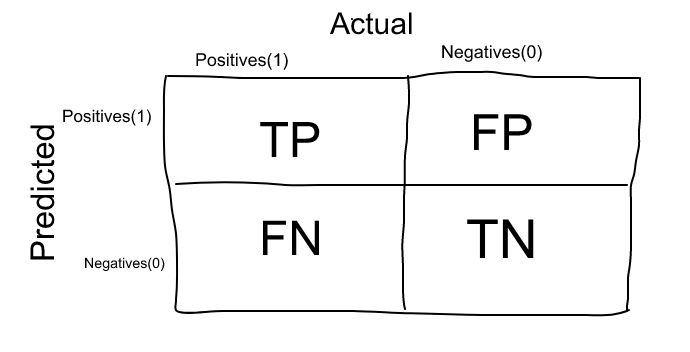
\includegraphics[scale=0.35]{./images/confusion_matrix}
    \caption{Confusion Matrix \cite{metrics}.}
    \label{fig:confusion_matrix}
\end{figure}
\begin{itemize}
    \item \textbf{True Positives (TP)} are cases when the actual class and the predicted are True (1)
    \item \textbf{False Positives (FP)} are cases when the actual class is False (0) and the predicted is True (1)
    \item \textbf{True Negatives (TN)} are cases when the actual class and the predicted class are False (True)
    \item \textbf{False Negatives (FN)} are cases when the actual class  is True (1) and the predicted is False (0)
\end{itemize}

\paragraph{Accuracy} Accuracy is the number of correct predictions made over all predictions.
\begin{equation}
Accuracy = \frac{TP + TN}{TP + FP + FN + TN}
\end{equation}

\paragraph{Precision} Precision is measure which tells us, what proportion of predicted positives are truly positives.
\begin{equation}
Precision = \frac{TP}{TP + FP}
\end{equation}

\paragraph{Recall} The recall metric tells us, what proportion of actual positives are correctly classified.
\begin{equation}
Recall = \frac{TP}{TP + FN}
\end{equation}

\paragraph{F1-Score} The F1-Score is the harmonic mean of precision and recall.
\begin{equation}
F1 Score = 2 * Precision * \frac{Recall}{Precision + Recall}
\end{equation}
%############

%############
\section{Analysis} \label{s_analysis}

\subsection{Data Exploration}
The dog images dataset has already been split into test, train, and valid sets. In total the dataset contains 8351 image files of 133 unique dog breeds. The images of the Udacity dog dataset have different dimensions, thereforethe images have to be resized, which is described in detail in \ref{s_methodology}. The LFW dataset contains 13234 images of 5749 unique individuals. Images in the LFW dataset have a dimension of 250x250 pixels.

\begin{figure}[h]
    \centering
    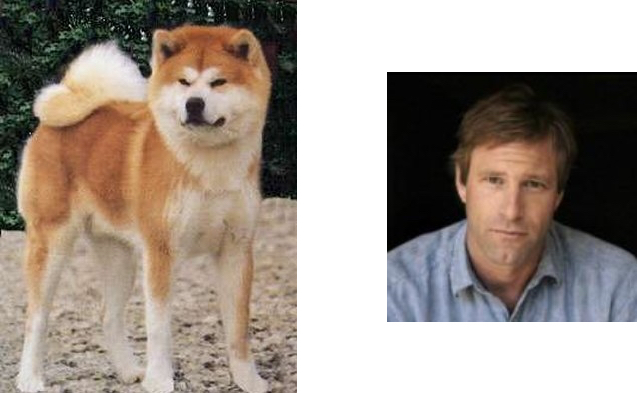
\includegraphics[scale=0.35]{./images/dataset_example}
    \caption{Example images from the datasets. The first images shows the Akita breed, the second image shows the actor Aaron Eckhart.}
    \label{fig:dataset_example}
\end{figure}

\subsection{Exploratory Visualization}
\begin{figure}[H]
    \centering
    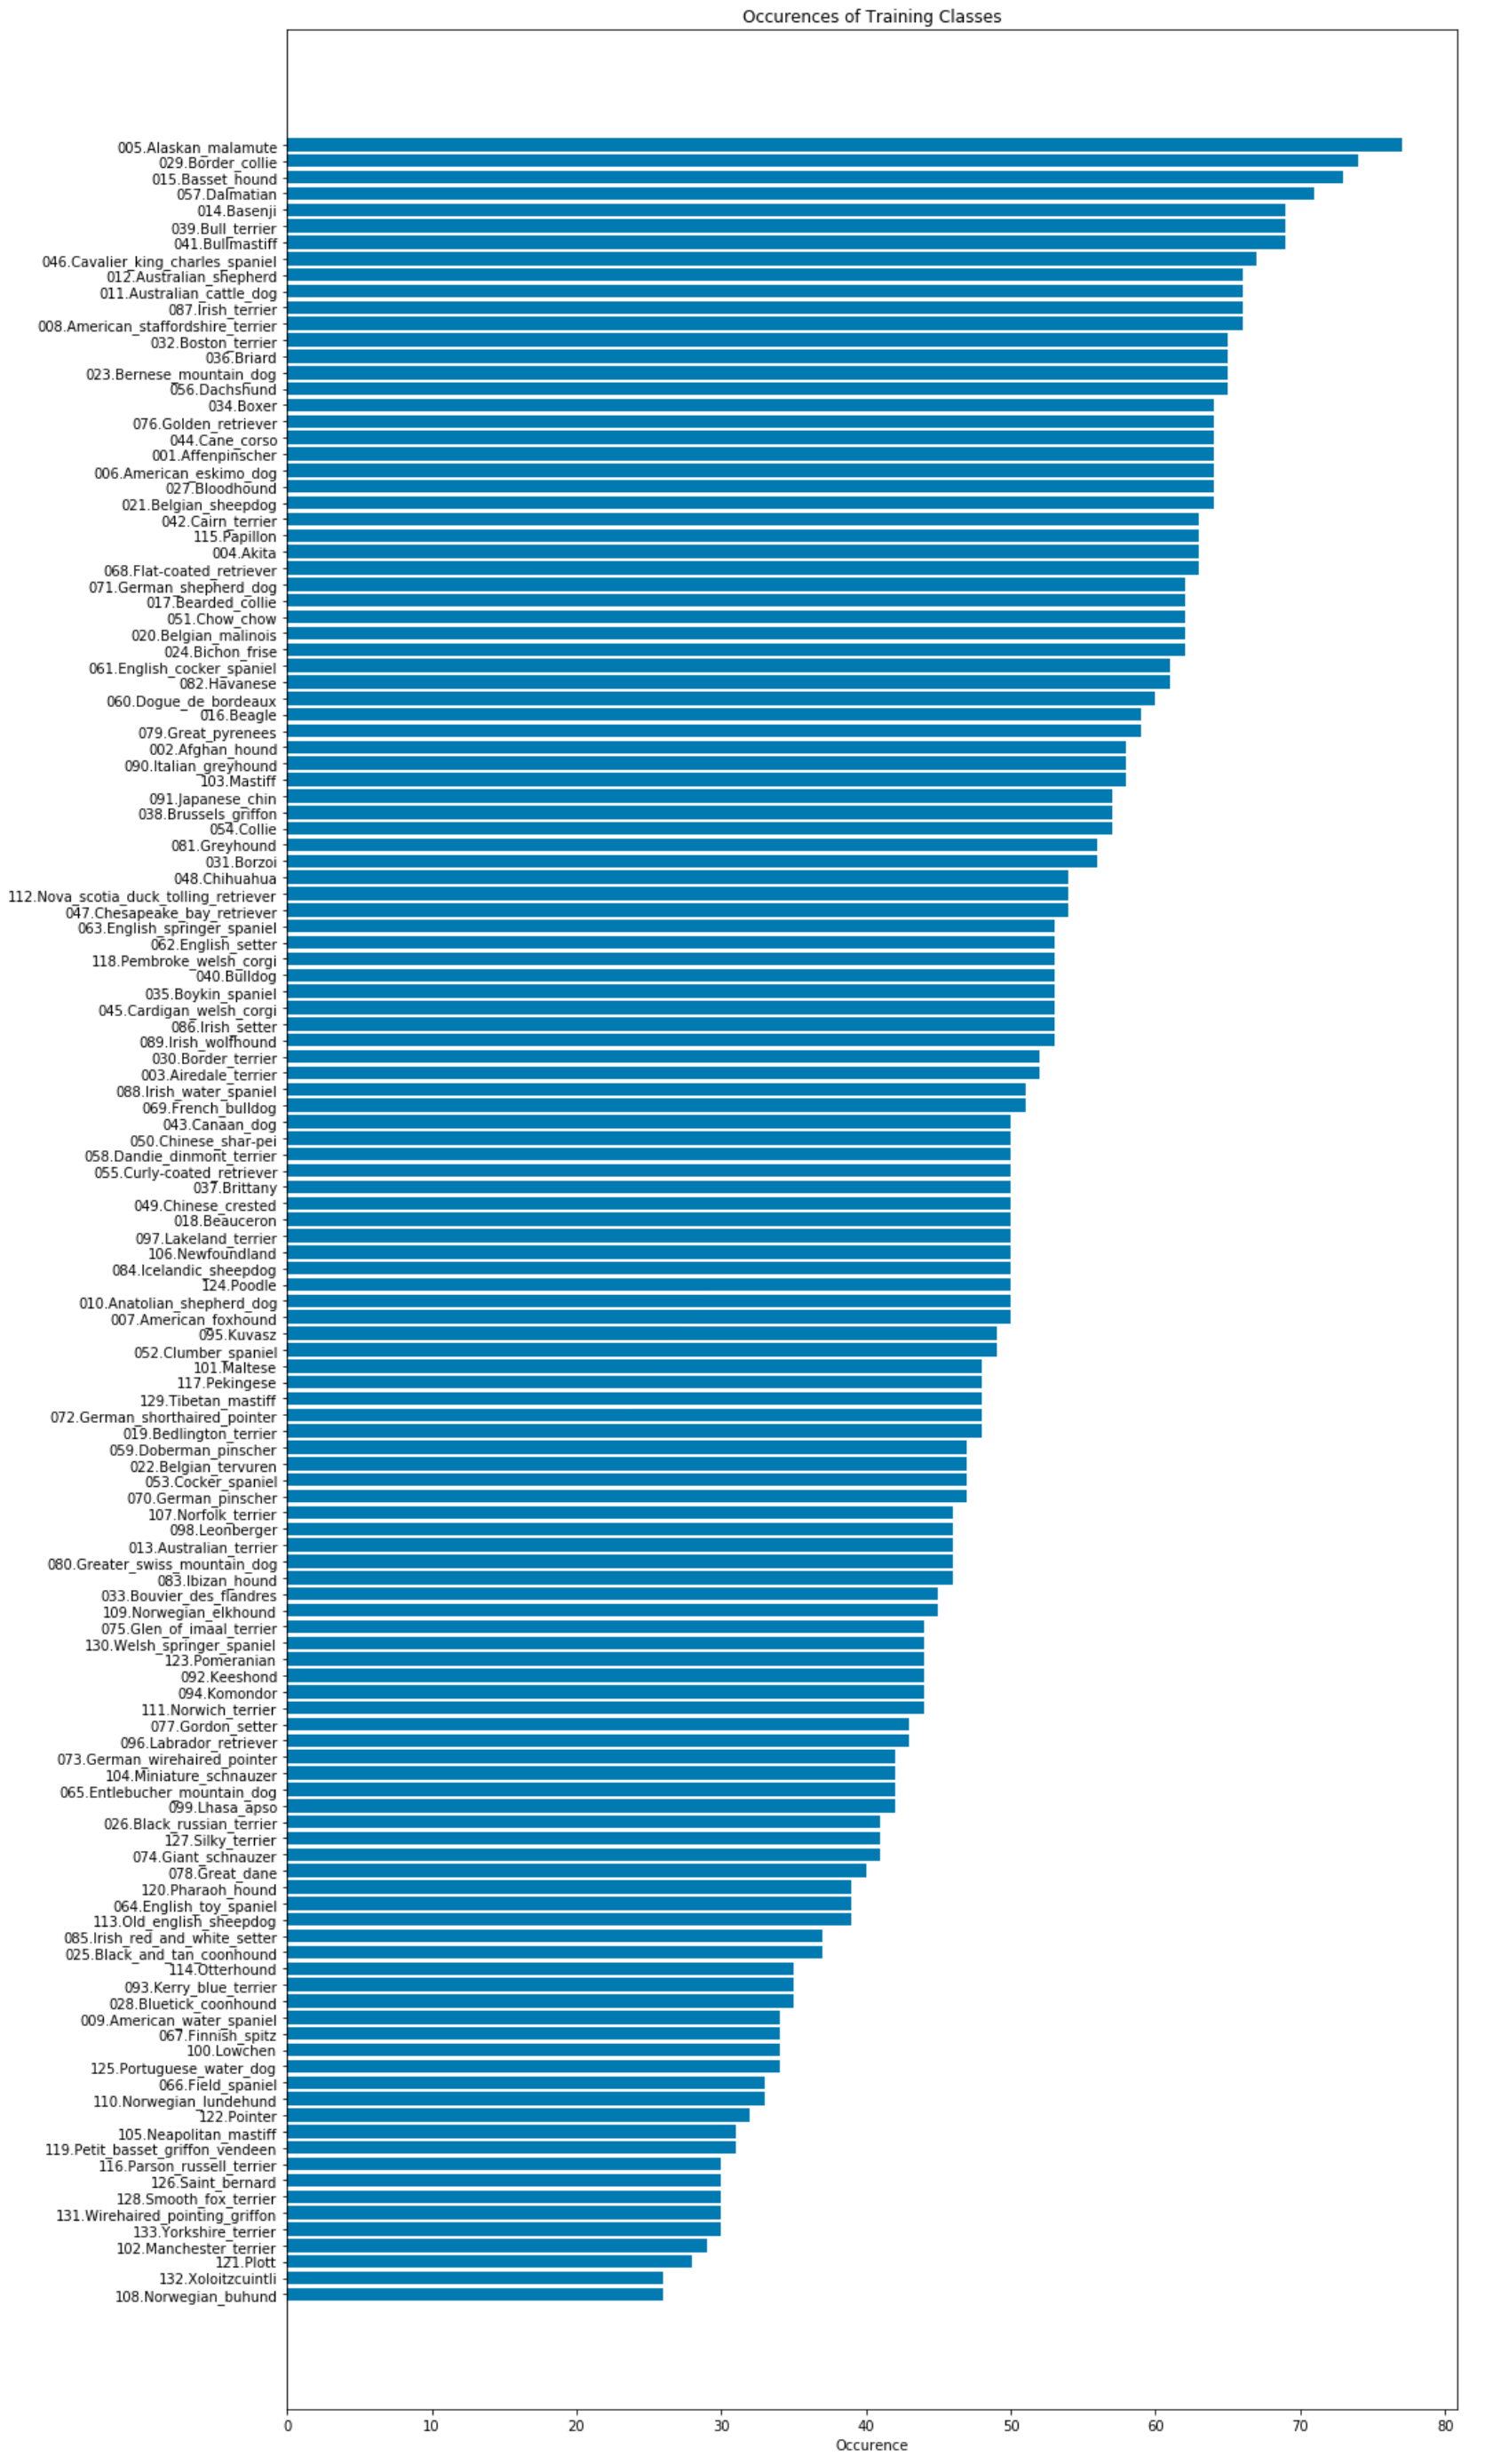
\includegraphics[scale=0.35]{./images/dog_breed_occurence}
    \caption{Visualization of dog breed occurences in the train dataset.}
    \label{fig:breed_occurence}
\end{figure}
The bar chart \ref{breed_occurence} shows the occurences of each individual dog breed in the train dataset. As the bar shows, the breeds are not evenly distributed. Therefore the CNNs of this project, will predict dog breeds with a higher occurence (e.g. Alaskan Malamute), better than breeds with a lower occurence (e.g. Norwegian Buhund).

\subsection{Algorithms and Techniques}
\paragraph{Face Detection} One part of the problem is to detect humans. Therefore a detector for human faces is needed. OpenCV provides the Haar Cascade classifier \cite{haar_cascade}. The classifier is trained from images with an machine learning approach based on a cascade function, to detect objects in images \cite{opencv}. OpenVC provides three different pretrained models to detect human faces: FrontalFaceAlt, FrontalFaceAlt2, FrontalFaceDefault. The comparison result showed, that FrontalFaceAlt is the best pretrained model for our use case. The model has an accuracy of 100\% for human faces.

\paragraph{Dog Detection} VGG-16 is a useful pretrained network to detect dogs. The VGG-16 network is recommended by the creators of the provided notebook. It is also possible to use other pretrained networks like Inception-v3 or ResNet-50. I decided to focus on VGG-16 for the dog detection, because in Transfer Learning, the ResNet-50 network will be used anyway.

\paragraph{Dog Classifier} This project has two mandatory tasks: Create a CNN from scratch and create a CNN using Transfer Learning. To create a CNN from scratch, the framework provided by the notebook is PyTorch. PyTorch is a machine learning library developed by facebook.\newline
For Transfer Learning I have decided to use the ResNet-50 pretrained network. The ResNet-50 network is trained with 152 layers on the ImageNet dataset and has won the 1st price on the ILSVRC 2015 classification task. Therefore, the ResNet-50 is the best fit for the problem of this project.

\subsection{Benchmark}
The benchmark requirements of this project are: The CNN made from scratch has to have an accuracy greater than 10\% and the Transfer Learning CNN has to have an accuracy greater than 60\%. The requirements are mandatory tasks from Udacity.\newline
There are no requirements about the dog detector or the human face detector. I have decided that an accuracy of at least 90\% has to be reached for these models.

%############
\section{Methodology} \label{s_methodology}

\subsection{Data Preprocessing}
The ResNet-50 network is trained with images of a 224x224 dimension. Therefore I decided to use that image size for the network I have to create from scratch. I will also use the same values for image normalization parameters like torchvision. The torchvision normalization parameters are:
\begin{itemize}
    \item \textbf{mean:} [0.485, 0.456, 0.406]
    \item \textbf{std:} [0.229, 0.224, 0.225]
\end{itemize}
According to these parameters, all input images will be preprocessed like the following:
\begin{enumerate}
	\item Resize to 224x224 with center crop
	\item Normalize with torchvision mean/std values
\end{enumerate}

The training data will be augmented, because it will increase the diversity of the test data, without adding new images and prevents overfitting. I decided to augment the images with a random horizontal flip and random rotation. Only horizontal flipping is activated, because dogs cant be upside down. The training images will be preprocessed like the following:
\begin{enumerate}
	\item Randomly resize the image to 224x224 with center crop
	\item Random horizontal flip
	\item Random rotation of 10 Degrees
	\item Normalize with torchvision mean/std values
\end{enumerate}

\subsection{Implementation}

\subsection{Refinement}

%############
\section{Results} \label{s_results}

\subsection{Model Evaluation and Validation}

\subsection{Justification}

%############
\bibliographystyle{plain}
\bibliography{references}
%############


\end{document}